\subsection{Setup}
For this part we fixed the distance to 50cm since we only want to change the DIFS and CWMIN. We keep the same conditions of our setup as previously.

\subsection{Expectations}
Lowering the DIFS means that we decrease the minimum wait time between packets. So in theory with only one sender this should result in a higher throughput.
In contrary when increasing the DIFS our throughput should decrease.

The CWMIN is the minimum size of the contention window. If there is a collision the sender waits for a random time between CWMIN and CWMAX.
In theory, if we decrease the CWMIN our throughput should increase and vice versa as long as there is only one sending station.
If we would work with multiple stations a smaller contention window would mean that the probability of multiple stations choosing the same value is higher and therefore more collisions happen and less throughput is achieved.

\subsection{Results}
The changes in DIFS result in a variation of the throughput as expected.
In our measurements we could not see an influence of alternating CWMIN.
The impact is probably not strong enough and would require further testing with modifying CWMAX as well.

\begin{figure}[htp]
\centering
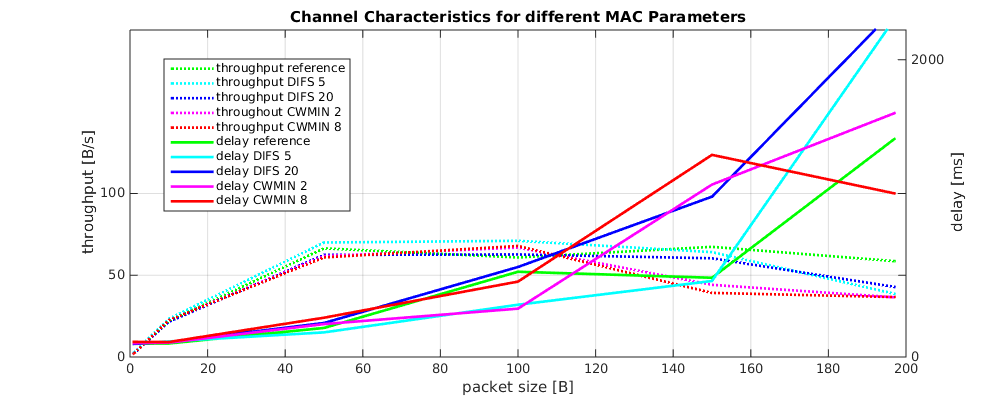
\includegraphics[width=\textwidth]{../img/plot_mac_parameters.png}
\caption{VLC channel characteristics for differing package sizes and distances}
\label{fig:chanchar}
\end{figure}